\chapter{Analysis techniques}

\section{General strategy for searching for four top quarks \label{sec:Strategy}}

The LHC has been said to be a ``top factory'' due to the large cross sections for \ttbar production at 8 TeV and 13 TeV, 253~pb and 831~pb respectively. Hence most analyses within the CMS collaboration which work on top quark physics study \ttbar production. Each of the top quarks will decay to a W boson and a b quark and the final state of the process in the detector is defined by whether the W boson decays leptonically into a lepton and neutrino or hadronically into two quark jets. The standard strategy is to require two b-jets to be present in the event and 0, 1, 2 leptons depending on the final state defined as \emph{all-hadronic}, \emph{semi-leptonic} and \emph{dileptonic} respectively where 6, 4 or 2 jets are required. 

\begin{figure}[ht!]
\centering
    \includegraphics[width=0.7\textwidth]{images/Analysis/Ttbar_decay_channels.png}
    \caption{The possible decay channels for \ttbar production}
    \label{fig:ttbarDecay}
\end{figure}
%picture from wiki By Nazar Bartosik - http://bartosik.pp.ua/hep_sketches/tt_decay_channels, CC BY 4.0, https://commons.wikimedia.org/w/index.php?curid=49739344

Each selection of b-jets, leptons and total number of jets in the event will not be $100\%$ efficient which means not all \ttbar events will be captured within the selection. As the rate of \ttbar production is so high at the LHC, this is satisfactory as the total number of events is still high enough to have statistically relevant studies.\\

The strategy for selecting \tttt events while suppressing the selection of background processes is similar to the \ttbar selection but with the selection of additional two jets. The small cross section for \tttt production, 1.3~fb at 8~TeV and $\approx$~9~fb at 13~TeV dictates the selection. It would be preferential to require 4 b-jets in the selection to obtain the highest signal to background ratio, however as b-tagging is $\approx70\%$ efficient, this would have a detrimental effect on the overall amount of \tttt found in the selection due to some b-jets not being identified correctly or being within the acceptance of the detector. Similarly, it is not possible to require the total number of jets in a \tttt final state as some of the jets may not be within the acceptance of the detector. However, it will be discussed in section~\ref{sec:Cats} how a looser selection can be used to an advance to constrain the main background process.

This thesis will mainly focus on the single lepton channel where only single muon and single electron final states are considered. As can be seen from~\ref{fig:ttttDecay}, the single lepton channel represents the largest branching ratio or four top quark decay channel. The dilepton channel, which has the second largest branching ratio will also briefly be discussed in chapter~\ref{c:Run2} as it was combined with the single lepton channel to achieve an increased sensitivity on the analysis. In the dilepton channel only final states with muons and electrons were considered.

\begin{figure}[ht!]
\centering
    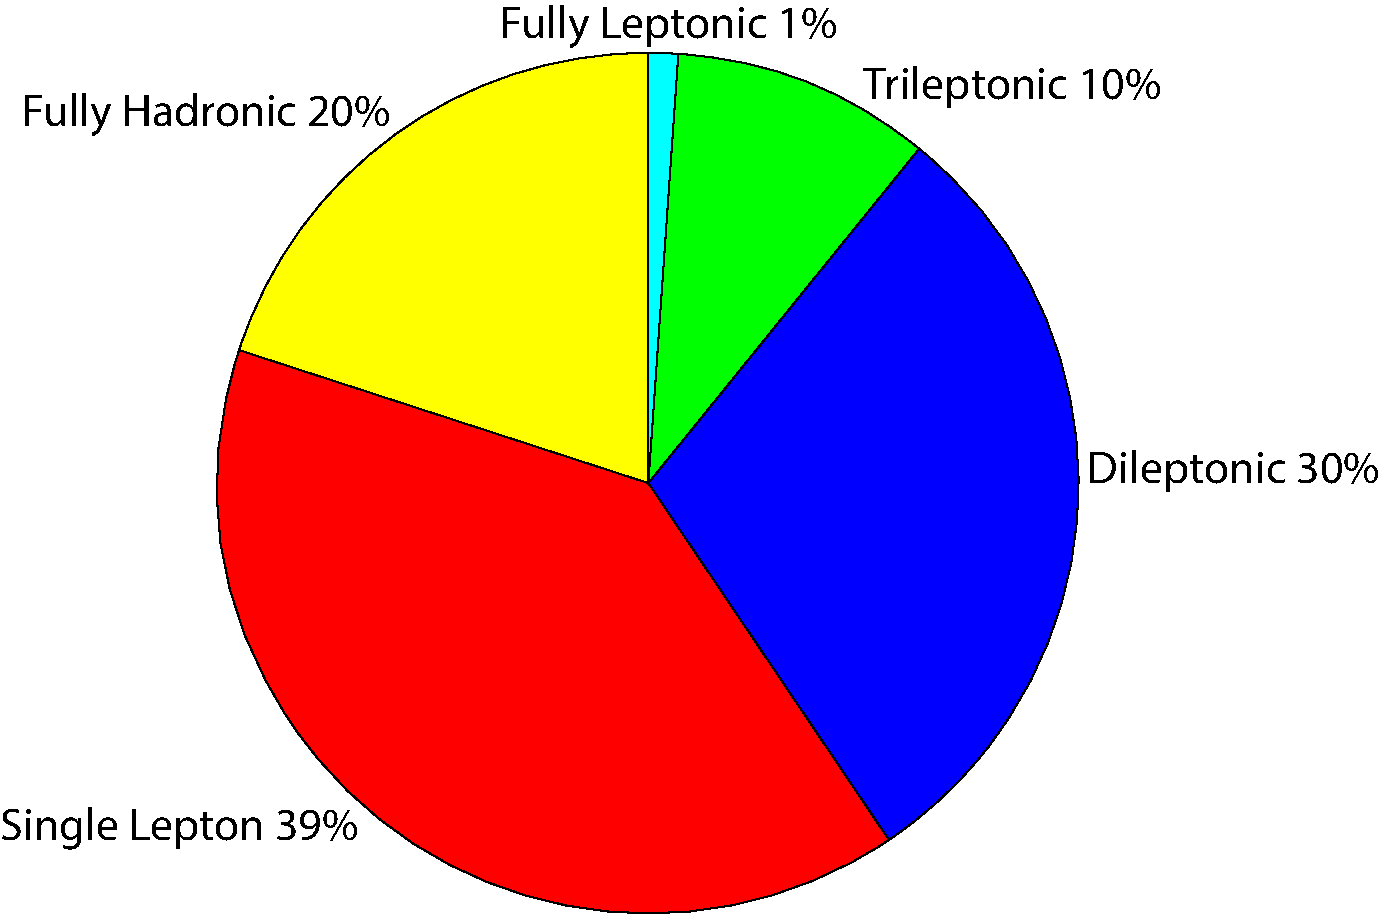
\includegraphics[width=0.5\textwidth]{images/Analysis/FourTopBR.pdf}
    \caption{The possible decay channels for \tttt production}
    \label{fig:ttttDecay}
\end{figure}




\section{Calibrations of the simulation}
\label{sec:Calibrations}
Many of the parameters which go into making simulation for each particle physics process are not precisely known therefore they are tuned to produce the simulation which best matches the data observed. This simulation will still have discrepancies from data which can be measured and accounted for by producing \emph{scale factors} which are combined and adjust the weight of each event in the simulation such that the overall distributions more closely matches data. 


\subsection{Pileup modelling}
\label{sec:pile-up}
The distribution of the number of primary vertices varies between data and simulation. This can be taken into account by looking at the number of events for each number of primary vertices in data and simulation and applying the scale factor, $SF_{PU}\left( i \right)$ to simulation, where \emph{i} is the number of vertices.

\begin{equation}
SF_{PU}\left( i \right) = \frac{N_{events}^{Data}}{  N_{events}^{simu}} 
\label{eqn:PUSF}
\end{equation}

\subsection{b tag modelling}

There are significant differences between b tagging efficiencies measured by CMS in data and the efficiencies as measured in simulation as it is difficult to simulate the fragmentation and hadronisation of b-quarks. 
The b-tagging efficiencies are measured for each of the CSVL, CSVM, and CSVT working points in bins of \pt and $\eta$. Depending on which working point was used in an analysis a scale factor, $SF(\eta, P_{T})_{i}$,  can be applied to the simulation for each jet which is dependent on the \pt, $\eta$ and flavour of the jet, shown in equation~\ref{eqn:sfbtagnorm}, where $\epsilon(\eta , \pt)^{data}_{i}$ is the efficiency for correctly identifying a b-jet in data and $\epsilon(\eta , \pt)^{simulation}_{i}$ is the efficiency for correctly identifying a b-jet in simulation.

\begin{centering}
\begin{equation}
SF(\eta, P_{T})_{i} = \frac{\epsilon(\eta , \pt)^{data}_{i}}{\epsilon(\eta , \pt)^{simulation}_{i}}
\label{eqn:sfbtagnorm}
\end{equation}
\end{centering}
Separate scale factors are defined by b and light (u, d, s, g) jets. Scale factors for c jets are taken to be the same as for b jets. A weight, $\omega_{btag}$ is applied to simulated events in order to correct for the expected difference between the efficiency in data and simulation. The method proceeds by defining the probability of an event in simulation producing a given number of tagged and untagged jets, P(MC),:

\begin{centering}
\begin{equation}
P(MC) = \prod_{tagged jets}\epsilon_{i} \times \prod_{untagged jets}(1- \epsilon_{i})
\end{equation}
\end{centering}
where $\epsilon_{i}$ is the efficiency of tagging a jet flavour $i$ with the CSV criterion. While the probability of an event in data producing a given number of tagged and untagged jets, P(DATA), is defined as follows:


\begin{centering}
\begin{equation}
P(DATA) = \prod_{tagged jets}SF_{i}\cdot\epsilon_{i} \times \prod_{untagged jets}(1- SF_{i}\cdot\epsilon_{i})
\end{equation}
\end{centering}
where SF is the appropriate scale factor for a jet of flavour $i$. 

An overall weight to be applied to each event depending on the jet content can be derived from these scale factors using the formula in~\ref{eqn:weightbtagnorm}. This weight, $\omega_{btag}$, must be applied to the selected simulation events in order to predict the correct event yield in data.

\begin{centering}
\begin{equation}
 \omega_{btag} = \frac{P(DATA)}{P(MC)}
 \label{eqn:weightbtagnorm}
\end{equation}
\end{centering}


Alternatively, the measurements at each working point can be used to fit the shape of the CSV distribution and provide scale factors in bins of \pt and $\eta$ for each jet flavour. Therefore the scale factors for each jet can be derived from the \pt and $\eta$, CSV discriminator value and for each jet flavour as seen in equation~\ref{eqn:btagcsv}. For this method, the jet flavours are defined as heavy for bottom quarks and light for u, s, d, g whilst c-quarks are given $\textrm{SF} = 1$. Further details of the CSV reshaping can be found in Ref.~\cite{CMS-NOTE-2013-130}.

\begin{equation}
\textrm{SFjet}_{\textrm{B}} \left(\textrm{CSV},\pt,\eta \right) = \frac{\textrm{Data} - \textrm{MC}_{\textrm{A}}}{\textrm{MC}_{\textrm{B}}} ~~;~~ \textrm{A, B = heavy flavour, light flavour or vice versa}
\label{eqn:btagcsv}
\end{equation}

An event weight can be derived by taking the product of the per-jet scale factors as seen in equation~\ref{eqn:btagcsvtot}.

\begin{equation}
\textrm{SF}_{\textrm{total}} = \prod_{i}^{\njets}\textrm{SFjet}_{i}
\label{eqn:btagcsvtot}
\end{equation}

\subsection{Heavy flavour jet modelling}
There is a discrepancy between data and simulation in the distribution of the number of b-tagged jets (\nbtags) at higher numbers of b-tags which suggests that the amount of heavy flavour jets in \ttbar events is incorrectly simulated. The extra jets can come from processes such as gluon splitting pair-producing \bbbar in \ttbar events. These \ttbb events are most likely to resemble to features of the \tttt signal events and so it is essential that the proportion of them in simulation is correctly modelled.
The ratio of $R=$\heavyflavour was measured by CMS to be $2.2 \pm 0.3 \left( \textrm{stat.} \right) \pm 0.5 \left(\textrm{sys.} \right)\% $ ~\cite{Khachatryan2015132} at $\sqrt{s} =$ 8~TeV and to be $2.2 \pm 0.3 \left( \textrm{stat.} \right) \pm 0.6 \left(\textrm{sys.} \right)\% $ ~\cite{CMS-PAS-TOP-16-010} at $\sqrt{s} =$ 13~TeV. To incorporate this ratio into the analysis, the MC truth information of the \ttbar$+$jets (MC) sample is used to split the sample into \ttbb, \ttcc and \ttll, where l denotes light quarks and gluons (\cPqu, \cPqd, \cPqs, \cPg). Weights are applied to each sub-sample to match the measured ratio whilst preserving the total number of \ttbar events.

\subsection{Lepton modelling}
Due to a difference between data and simulation in the efficiency of lepton identification, isolation, reconstruction and triggering, a weight is applied to events which is dependent on the selected leptons $\eta$, $\pt$ and lepton flavour. The scale factors for each source of efficiency are designed to be multiplicative and the final event weight can be found in equation~\ref{eqn:leptonW}

\begin{equation}
\omega_{lepton} = SF_{iso}\times SF_{id}\times SF_{reco}\times SF_{trig}
\label{eqn:leptonW}
\end{equation}

\subsection{Top \pt modelling}

There is a known problem in the modelling of the top quark \pt spectrum where the top quarks found in data appear tend to be lower in \pt than simulation. A scale factor can be derived as a function of the \pt of the top as generated in the simulation before being reconstructed in the detector. The event weight is shown in equation~\ref{eqn:topptW}

\begin{equation}
\omega_{topPt} = SF_{top}\times SF_{anti-top}
\label{eqn:topptW}
\end{equation}

\subsection{Jet multiplicity modelling}
Good modelling of the jet multiplicity distribution up to a large number of jets (up to fifteen jets) in the main \ttbar background is highly important for this analysis because as the number of jets increase the signal to background ratio increases. Hence, the higher \njets multiplicity categories mentioned in section~\ref{sec:Cats} are where the highest sensitivity in separating the signal \tttt process and the background \ttbar process. It is essential that \ttbar is well modelled in this high jet multiplicity region. 
Particularly at 13 TeV the simulation was larger than data in the higher \njets bins. The value of $\alpha_S$ in the \ttbar Powheg+Pythia8 sample used in the analysis in chapter~\ref{c:Run2} is 0.137, however the best tune was observed to have a value of $\alpha_S=0.113^{+0.012}_{0.010}$. A scale factor was derived by CMS in order to improve the modelling of the \njets distribution. 

\section{Multi-jet background estimation}
\label{sec:QCDbackground}
The presence of multi-jet events within the signal region defined by the baseline selection is investigated in this section. \fxnote*{why?}{It is rare for multi-jet events to have a highly energetic undetectable particle}. Therefore, the $\MET$ distributions for multi-jet events typically peak at low values, not necessarily at zero as some jets may be outside of the acceptance of the detector or mis-measured. Due to the small number of events which pass the selection and the difficulty in simulating QCD events, it is not possible to use multi-jet simulation to estimate this background. In this case, a data-driven method known as the \fxnote*{ref?}{``ABCD method''} may be used. This method proceeds by selecting two uncorrelated variables from the object or baseline selection and defining three control regions (A,B,C) and one signal region, D, in the 2-dimensional phase space of these variables as shown in Fig.~\ref{fig:ABCDdiagram}. A selection is made in each variable which defines one quadrant of the phase space as the signal region.  The event variable \MET and the lepton variable RelIso were selected as they are \fxnote*{uncorrelated proof??}{uncorrelated} where the signal is defined in a low RelIso and higher \MET region.\\

\begin{figure}[ht!]
\begin{center}
\subfloat{
\includegraphics[width=0.6\textwidth]{images/Analysis/ABCDdiagram.pdf}
\includegraphics[width=0.6\textwidth]{images/Analysis/ABCD2.pdf}
}
\hspace{0.2cm}
\end{center}
\caption{Illustration of ABCD method}
\label{fig:ABCDdiagram}
\end{figure}

% \begin{equation}
% \frac{\textrm{N}^{\textrm{B}}_{\textrm{multi-jet}}}{\textrm{N}^{\textrm{A}}_{\textrm{multi-jet}}} = \frac{\textrm{N}^{\textrm{C}}_{\textrm{multi-jet}}}{\textrm{N}^{\textrm{D}}_{\textrm{multi-jet}}}
% \label{N-multi-jet}
% \end{equation}

The backgrounds which are modelled well in simulation are subtracted from the data, in terms of number of events in each bin. This should in theory leave only QCD multijet events remaining and so the number of events in the signal region can be estimated from the equation in Fig.~\ref{fig:ABCDdiagram}. This method does have some dependence on the simulation and an assumption that the other backgrounds are well modelled. The uncertainty on this assumption can be taken into account by varying the main \ttbar background by its main source of uncertainty. 


\section{Multi-variate analysis techniques}

Four top quark production events are very rare at the energies of $\sqrt{s} = $ 8~TeV and 13~TeV studied in this thesis. Typically within the selection defined in Section~\ref{sec:Strategy} the main background is \ttbar production which is $\approx$ five orders of magnitude larger than the \tttt signal. In this type of analysis where the background and signal can be similar in many variable and the signal is so rare, it can be advantageous to use multivariate analysis (MVA) methods to increase the signal to background separation. The main MVA method used in this thesis is \emph{Boosted Decision Trees} (BDT) where more details of this algorithm and it's specific use in this analysis are given in the subsequent sections.


\subsection{Boosted Decision Trees}
\label{sec:BDT}

To start with, the simpler concept of a single Decision Tree will be considered. Decision trees are used to maximise the separation between a signal sample and a background sample by looking at a set of variables which each have some initial separation; a training sample for each is provided to the algorithm. 

One can define the purity at each node as $P=\frac{S}{S+B}$. Another useful measure is the \emph{gain} at each node. The particular metric of gain used in this analysis is the commonly used \emph{Gini Index} which is defined as $Gini = P\cdot\left(1-P\right)$. A high Gini Index suggests the node contains a relatively equal amount of signal and background whereas a low Gini index shows that the node contains more of either signal or background. 
The goal is to scan across each variable and find the cut and the associated variable which maximises the \emph{separation gain} ($S_{G}$) as defined in equation~\ref{eqn:SepGain}. This process is iterated upon until a predefined end condition such as the maximum depth of the tree or the minimum number of events in a node.


% \begin{equation}
% P=\frac{S}{S+B}
% \label{eqn:Purity}
% \end{equation}

% \begin{equation}
% Gini = P\cdot\left(1-P\right)
% \label{eqn:Gini}
% \end{equation}

\begin{equation}
S_{G} = Gini(\textrm{parent}) - Gini(\textrm{child 1}) - Gini(\textrm{child 2})
\label{eqn:SepGain}
\end{equation}

\begin{figure}[h!]
\begin{center}
\subfloat{
\includegraphics[width=0.67\textwidth]{images/Analysis/BDTFlow.png}}
\hspace{0.2cm}
\end{center}
\caption{Illustration of a single decision tree of depth = 3~\cite{2007physics3039H}.}
\label{fig:alphaSuncorrected}
\end{figure} 

It has been found that using an ensemble (usually several hundred) of smaller decision trees of depth = 2 or depth = 3 is preferable to using one large decision tree as it can minimise \emph{overtraining}, ie. the propensity to train to the specific features of the training sample rather than the general trend. 

The first tree begins as a normal decision tree as described above and it terminates when it reaches the max depth defined. The error rate of the tree is defined as the number of events incorrectly classified divided by the total number of events. The events which were incorrectly categorised are weighted according to equation~\ref{eqn:ErrorWeight} where $\alpha$ is the \emph{boost weight} and $\beta$ is the learning rate which can be adjusted by the user. The idea is that in the next iteration of a tree the incorrectly classified are considered more heavily. 

\begin{equation}
\alpha^{\beta} = \left( \frac{\textrm{1-err}}{\textrm{err}}  \right)^{\beta}
\label{eqn:ErrorWeight}
\end{equation}

This process is repeated until the max number of trees has been reached, as defined by the user. 

A discriminator value, $y_{BDT}$, is defined by summing the response from each tree and weighting each response such the trees with low error rates are considered more than trees with high error rates. The response from each individual tree, \emph{t}, is defined as $h\left(\textbf{x}\right)$ where $h\left(\textbf{x}\right) = +1 \textrm{ for signal and} -1 \textrm{ for background}$ and $\textbf{x}$ is the set of input variables. 

\begin{equation}
y_{BDT} = \frac{1}{Ntrees} \cdot \sum_{t}^{Ntrees} \ln \left(\alpha_{t}\right) \cdot h_{t}\left(\textbf{x}\right)
\end{equation}

Values of $y_{BDT}$ which are closer to +1 (-1) are considered to be more signal-like (background-like).

\subsection{Reconstruction of hadronic top quarks}

In \tttt there are three hadronically decaying top quarks in the single lepton channel and one hadronically decaying top quark in the semi-leptonic \ttbar final state. Equivalently in the dilepton channel there are two (zero) hadronically decaying top quarks in \tttt (\ttbar). Therefore reconstructing top quarks from their hadronic decay products should be a powerful way to separate the signal and background processes. The jets which are additional to the hard process in \ttbar are likely to come from initial or final state radiation (ISR or FSR) or from pileup, hence it should not be possible to reconstruct a hadronic top quark from these additional jets. Due to the large number of jets within the selection, it is combinatorial challenge to find the right combination of jets which originated from a top quark. This motivates using multivariate analysis in order to rank each combination of three jets (tri-jet) according to which is most likely to be the combination that originated from a real hadronically decaying top quark.
A training sample from \ttbar events is provided to the BDT where the Monte Carlo truth information is used to classify whether a tri-jet combination was a \emph{good} combination which originated from a top quark or a \emph{bad} combination which is formed from random jets. The following variables were selected for use within the BDT:\\
\textbf{Tri-jet invariant mass} - Good tri-jet combinations should have an invariant mass distribution which peaks around the top mass.
Bad tri-jet combinations will have a much broader distribution. \\
\textbf{Di-jet invariant mass} - The di-jet combination is formed from the two jets with the smallest \DR separation. The invariant mass distribution should peak around the W mass for good tri-jet combinations.\\
\textbf{\ptrat} - This is the ratio of the vectorial \pt to the scalar sum of the \pt of the jets in the tri-jet combination. This is likely to be smaller in a random combination of jets where the vectoral \pt of each jet will cancel out more than in a good tri-jet combination.\\
\textbf{\DPTW} - This is the \Dphi separation between the tri-jet and di-jet system which should be smaller in good tri-jet combinations.\\
\textbf{\DPTb} - This is the \Dphi separation between the tri-jet and remaining jet not included in the di-jet system which should be smaller for good tri-jet combinations.\\
\textbf{\CSVj} - For the jet not used in the di-jet system, the CSV b-tagging discriminator value is used. If the di-jet system correctly identifies that quark-jets coming from a W boson decay then the remaining jet in a good tri-jet combination should be a b-jet and hence will have a higher CSV b-tagging discriminator than a typical randomly selected jet.\\

The BDT algorithm is trained on the six variables above. It produces a discriminator value for each tri-jet combination. Higher BDT discriminator values are associated with being more likely to have come from a top quark. Each tri-jet combination is ranked according to the BDT discriminator value. In the dilepton channel the value for the highest ranked tri-jet, known as BDT$_{tri-jet1}$, can be used as a discriminating variable between \tttt and \ttbar. In the single lepton channel the three jets which make up the highest ranked tri-jet combination and removed from the collection and jets and the process is repeated. The discriminator value of the next highest ranked tri-jet, BDT$_{tri-jet2}$, in this reduced jet collection can be used to distinguish between \tttt and \ttbar in the single lepton channel as semi-leptonic \ttbar should have only one hadronically decaying top quarks and hence BDT$_{tri-jet1}$ is not a powerful variable to use.

\subsubsection{Reduced Variables}
As mentioned above, BDT$_{tri-jet2}$ is calculated from a reduced jet collection where the three jets from the highest-ranked tri-jet are removed from the jet collection. In \ttbar events, the removal of the jets most likely to form a true top quark leave softer jets remaining in the reduced jet collection, usually from ISR, FSR or PU rather than the hard process of \ttbar production. In \tttt events the removal of the leading hadronic top quark candidate potentially leaves behind two additional hadronic top quarks, where some of the jets may not be reconstructed but there should still be harder jets from the hard process than what remains in \ttbar events. Therefore some discriminating variables can be formed from the reduced jet collection, as follows:

\textbf{HT$_{X}$} - This is the \HT of the reduced event which should be higher for signal \tttt events.\\
\textbf{\sumjetmassX} - Invariant mass of all jets contained in the reduced event which should be higher for signal \tttt events..

\subsection{Event-level BDT}

\section{Limit setting}

\subsection{Categorisation}
\label{sec:Cats}




